\section{Local Fourier Spectral Filters}
\label{sec:lfsfilter}

\subsection{Desired Properties}
\label{sec:lfs_properties}
When designing the \gls{lfs} Filters presented in this paper, we considered the following properties as desirable:
\begin{enumerate}[1. ]
\item The filter should have spectral interpretation so there is control over the physical scales being smoothed
\item \label{item:local_stencil} The filtering operation must have a local stencil: only interior and boundary solution values can be used to filter the solution in the interior of the element
\item \label{item:filt_bc}The filter should preserve boundary conditions
\item \label{item:filt_bi}Filtering the solution at the interior points should be influenced by the solution values at the element's boundary
\item \label{item:influence}The influence of a boundary point on the internal point being filtered should be inversely proportional to the distance between them
\item To limit computational cost, the filter should be applied in the reference domain and involve matrix-vector multiplications exclusively

\item \label{item:generalizability}Filtering strategy should be generalizable to any type of element in unstructured grids

In the early stages of the filter design, we noted that Properties \ref{item:filt_bc} and \ref{item:filt_bi} could be overly stringent, so we re-phrased them as the following, more relaxed condition:

\item \label{item:coplanar}If solution values at the boundary lie on a hyperplane in the space of spatial coordinates and solution values, the filtering operation should bring the internal solution values closer to such plane. In other words, if the solution values at the boundaries can be determined from a linear function of their location, the filter should bring the internal solution values closer to satisfying such linear function.
\end{enumerate}



Condition \ref{item:coplanar} may not allow a filtered solution to satisfy the boundary conditions always. Nevertheless, in the limit of infinite mesh refinement the solutions at the boundary of every element will be coplanar, even in the presence of shocks in the \gls{ns}  equations. Hence, Condition \ref{item:coplanar} satisfies conditions \ref{item:filt_bc} and \ref{item:filt_bi} asimptotically. This re-formulation was inspired by the \gls{eled}  property of the \gls{jst}  scheme\cite{jameson1981numerical} for finite volume methods. Whether or not (some) \gls{lfs} filters satisfy \gls{eled}  properties shall be left for a future study.

%At this point it is important to note the main difference between the filters being proposed here and the commonly used modal filters\cite{kanevsky2006idempotent}. Modal filters are not influenced by the values of the solution at the boundary points. Therefore, if an element is experiencing aliasing, a modal filter will not necessarily ``nudge" the internal solution values towards continuity with its neighbors. In addition, in the limit of mesh refinement, modal filtering might not enforce an element's boundary conditions.

\subsection{Mechanics of \gls{lfs} Filters}

The core idea of the \gls{lfs} filtering technique is that the solution is filtered with a matrix whose entries depend on the element interface values, the basis functions of the solution, and a selected Fourier filtering kernel.

Suppose we wish to filter the scalar field $v$ inside an arbitrary element. This field could be density, momentum in a specific direction, or energy. We can represent $v$, as usual, as a weighted sum of basis functions.
\begin{equation}
\label{eqn:polyexp}
v(\bxi) = \sum^{N_s}_{i=1} v_i \phi_i(\bxi),
\end{equation}
where $v_i$ is the \ith weight, $\bxi$ is a vector of coordinates in a reference domain, and $\phi_i(\bxi)$ is the \ith basis function.

The key component of the \gls{lfs} technique is that the Fourier filtering operation over the element is approximated at each internal point $i$ with coordinates $\bxi_i$. Suppose we wish to use filtering kernel $G(\bxi)$ to filter $v(\bxi)$, then the filtered value at internal point $i$ becomes
\begin{equation}
\label{eqn:convolution}
\begin{split}
\bar{v}_j &= (G \ast v)(\bxi_j)\\
&= \int_{\mathbb{R}^d} G(\bxi_j - \bxi)v(\bxi)d\bxi\\
&= \int_{\mathbb{R}^d} G(\bxi_j - \bxi)\l(\sum^{N_s}_{i=1} v_i \phi_i(\bxi)\r)d\bxi\\
&= \sum^{N_s}_{i=1}v_i\int_{\mathbb{R}^d} G(\bxi_j - \bxi)  \phi_i(\bxi)d\bxi,\\
\end{split}
\end{equation}

where $\Omega$ is the entire problem domain, not just the element domain, $N_s$ is the number of solution points, and the overbar means the quantity is filtered. Filtering over the entire domain would be computationally expensive, but would certainly smoothen the solution field and can be done while maintaining the order of accuracy of the underlying numerical scheme\cite{mirzaee2012efficient,steffen2008investigation,walfisch2009one}. In order to use only a local (element-wise) stencil, it is possible to break the integration as follows
\begin{equation}
\label{eqn:brokenint}
\int_{\mathbb{R}^d} G(\bxi_j - \bxi)  \phi_i(\bxi)d\bxi = \int_{\Omega_n} G(\bxi_j - \bxi)  \phi_i(\bxi)d\bxi + \int_{\mathbb{R}^d \backslash \Omega_n} G(\bxi_j - \bxi)  \phi_i(\bxi)d\bxi,
\end{equation}
where $\Omega_n$ is the domain of element $n$ (where the $\phi_i$ values are known) and $\Omega \backslash \Omega_n$ is the complement of $\Omega_n$ in $\Omega$. As $G$ and $\phi_i$ are defined in $\Omega_n$, it is possible to calculate the first integral in Equation \eqref{eqn:brokenint} analytically or via an adaptive quadrature algorithm like \texttt{quanc8}~\cite{forsythe1977computer}.

A design choice arises in defining $\phi_i$ in the domain $\Omega \backslash \Omega_n$. Asthana et al.~\cite{asthana2014} initially decided to let $\phi_i$ equal a constant in 1D elements, and a combination of constant and polynomial in quadrilaterals. Non-tensor-product elements became problematic for this kind of formulation. This paper presents a more generic filter design method based on the desired properties in Section \ref{sec:lfs_properties}.

Let us describe the mechanics of the two components of the integral in Equation \eqref{eqn:brokenint} in a subsection each. We can call the filter associated with the term $\int_{\Omega_n} G(\bxi_j - \bxi)  \phi_i(\bxi)d\bxi$ ``Internal Filtering Component" and the filter associated with the term $\int_{\mathbb{R}^d \backslash \Omega_n} G(\bxi_j - \bxi)  \phi_i(\bxi)d\bxi$ ``Boundary Filtering Component".

The filtering operation being sought follows this format
\begin{equation}
\label{eqn:filter_form}
\vec{\bar{v}} = \alpha\mat{T}\vec{v} + (1-\alpha)\mat{B}\vec{v^*},
\end{equation}
where $\mat{T}$ is the internal filtering component, as it acts on the solution at internal points $\vec{v}$, and $\mat{B}$ is the boundary filtering component, as it acts on the solution at boundary points $\vec{v^*}$, and $\alpha$ is a scalar between $0$ and $1$ that determines the relative influence the internal and boundary components have on the internal solution values.

\subsection{Internal Filtering Component}
There are two steps to the creation of the internal filtering component $\mat{T}$. First we create the filtering matrix with the spectral interpretation, and then we normalize it so if the quantity being filtered is a constant, the filter preserves the constant.
\subsubsection{Matrix formation}
It can be seen from the last line in Equation \eqref{eqn:convolution} that finding the vector of solution values filtered with the internal component can be posed as a matrix-vector multiplication:
\begin{equation*}
\label{eq:internal_matrix}
\begin{bmatrix}
\bar{v}_1 \\
\bar{v}_2 \\
\vdots\\
\bar{v}_{N_s} \\
\end{bmatrix} = 
\begin{bmatrix}
\int_{\Omega_n} G(\bxi_1 - \bxi)  \phi_1(\bxi)d\bxi &
\int_{\Omega_n} G(\bxi_1 - \bxi)  \phi_2(\bxi)d\bxi &
\cdots &
\int_{\Omega_n} G(\bxi_1 - \bxi)  \phi_{N_s}(\bxi)d\bxi\\
\int_{\Omega_n} G(\bxi_2 - \bxi)  \phi_1(\bxi)d\bxi &
\int_{\Omega_n} G(\bxi_2 - \bxi)  \phi_2(\bxi)d\bxi &
\cdots &
\int_{\Omega_n} G(\bxi_2 - \bxi)  \phi_{N_s}(\bxi)d\bxi\\
\vdots & \vdots & \ddots & \vdots\\
\int_{\Omega_n} G(\bxi_{N_s} - \bxi)  \phi_1(\bxi)d\bxi &
\int_{\Omega_n} G(\bxi_{N_s} - \bxi)  \phi_2(\bxi)d\bxi &
\cdots &
\int_{\Omega_n} G(\bxi_{N_s} - \bxi)  \phi_{N_s}(\bxi)d\bxi
\end{bmatrix}
\begin{bmatrix}
v_1 \\
v_2 \\
\vdots\\
v_{N_s} \\
\end{bmatrix}.
\end{equation*}

More compactly,
\begin{equation}
\label{eqn:filtmat}
\vec{\bar{v}} = \mat{F}\vec{v}
\end{equation}
we use over-arrow to denote column vectors.
Interesting choices for $G(\bxi)$ depend on a desired wavenumber threshold $h$:

\begin{enumerate}[I.]
\item Gaussian function:
\begin{equation}
G(\bxi) = h \exp{(h||\bxi||)},
\end{equation}
where $||\bxi||$ is a measure of the length of $\bxi$.
\item \label{item:multi_ind_func}Multidimensional indicator function:
\begin{equation}
G(\bxi) = h\mathrm{I}_{[0,1]}(h||\bxi||),
\end{equation}
where $\mathrm{I}_{[0,1]}(x) = 1 \text{ if } 0\le x\le 1$, and $0$ otherwise.
\item \label{item:sharp_spectral}Multidimensional sharp-spectral function:
\begin{equation}
\label{eq:sharp_spectral}
G(\bxi) = h||\bxi||^{-n/2}
J_{n/2}(h||\bxi||),
\end{equation}
where $J_\alpha$ is a Bessel function of the first kind and $n$ is the number of dimensions of $\bxi$.
\end{enumerate}

In these functions, the larger the value of $h$, the thinner the filter is in physical space, so the fewer wavenumbers it dampens. Note that as $h \rightarrow \infty$, $\mat{F}_{ij}  \rightarrow \phi_j(\bxi_i)$, so $\vec{\bar{v}} \rightarrow \vec{{v}}$. The integrals in Equation \eqref{eq:internal_matrix} can be evaluated to arbitrary accuracy with \texttt{quanc8}~\cite{forsythe1977computer} in a pre-processing stage.

\subsubsection{Enforcing Conservation of a Constant Quantity}
The requirement to preserve a constant can be posed in an equation as
\begin{align}
\bar{v}_i = \sum^{N_s}_{j = 1} \mat{F}_{ij} v_{\text{const}} = v_{\text{const}},
\end{align}
where $v_{\text{const}}$ is a constant scalar. As a result, each row of $\mat{F}$ must satisfy
\begin{align}
\sum^{N_s}_{j = 1} \mat{F}_{ij} = 1,
\end{align}
where $i = 1,\dots,N_s$.
This constraint can be enforced by dividing each row of $\mat{F}$ with the total sum of the row. More explicitly,
\begin{align}
{\mat{T}}_{ij} = \frac{\mat{F}_{ij}}{\sum^{N_s}_{k = 1} \mat{F}_{ik}},
\end{align}
where the normalized matrix ${\mat{T}}$ is the internal filtering component in Equation \eqref{eqn:filter_form}.

\subsubsection{Integration Domain}

The normalization of the matrix introduces a bias. As the integration is being performed in some reference domain $\Omega_n$, the integral $\int_{\Omega_n} G(\bxi_i - \bxi)  \phi_j(\bxi)d\bxi$ will tend to have a greater value when $\bxi_i$ is well inside the reference element. This is more evident when using the multidimensional indicator function (shown in \ref{item:multi_ind_func}) as the filtering kernel.

To ameliorate this bias, we have selected to perform the integration in a reference domain that is symmetric. With this precaution all integrals related to points close to a domain edge have a similar magnitude, and thus the filtering operation does not favor points close to some arbitrary edge over the others.

Figure \ref{fig:domain_example} illustrates the potential introduction of bias in triangular elements that use a right triangle as a reference element.

\begin{figure*}

\subfloat[Equilateral triangle domain\label{fig:equi_tri_domain}]{%
      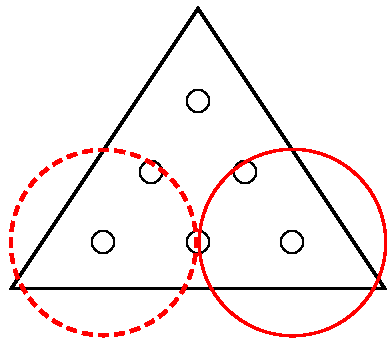
\includegraphics[width=0.45\textwidth]{\lfsdir/figs/equi_tri.pdf}
    }
    \hfill
    \subfloat[Right triangle domain\label{fig:right_tri_domain}]{%
          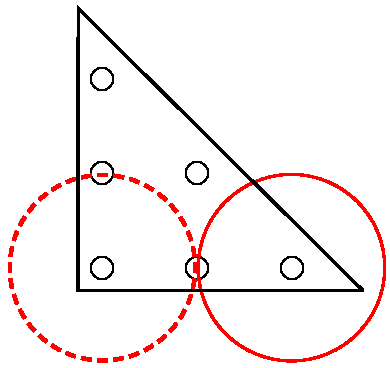
\includegraphics[width=0.45\textwidth]{\lfsdir/figs/right_tri.pdf}
        }
\caption{Using the same filter width in two different domains introduces different bias. The small, solid circles represent the location of solution points. The large circles represent the filter width acting on two specific internal points in two different domains. Integration is being performed in the area encompassed by the solid, straight lines.}
\label{fig:domain_example}

\end{figure*}

In practice, the basis functions $\phi_j(\bxi)$ may be defined in non-symmetrical elements. To simplify the evaluation of the integral, the definition of the norm in the filtering kernel $G(\bxi)$ can be modified so the curve drawn by $||\bxi -\bxi_0|| = 1$ in the non-symmetric reference element would map to a circle in a symmetric reference element.

In the case of a triangle, the basis functions are defined in a right triangle with vertices $[-1,-1], [1,-1],[-1,1]$.

By defining the norm in this right triangle as follows
\begin{equation}
\label{eqn:rect_norm}
||\bxi||^2_{rt} = \bxi_1^2 + \bxi_2^2 + \bxi_1\bxi_2,
\end{equation}
$||\bxi -\bxi_0||_{rt} = 1$ maps to a circle in the equilateral triangle with vertices $[-1,-1],[1,-1],[0,\sqrt{3}-1]$. Figure \ref{fig:mapping} sketches this mapping. $||\cdot||_{rt}$ is the norm defined in the right triangle.


\begin{figure}\centering
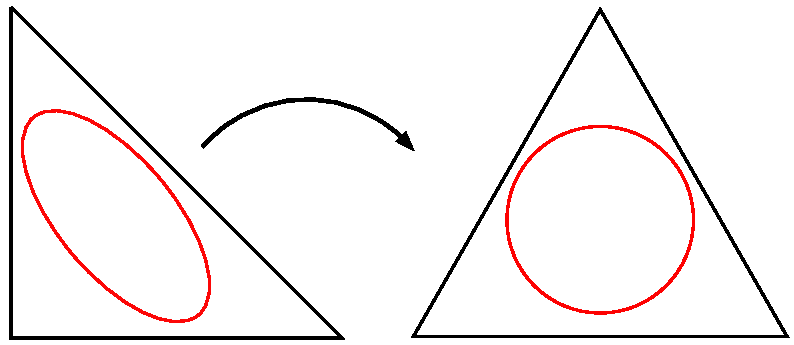
\includegraphics[width = 0.75\textwidth]{\lfsdir/figs/mapping.pdf}
\caption{Sketch of ellipsis $||\bxi -\bxi_0||_{rt} = 1$ defined in the right triangle domain maps to a circle in the equilateral triangle domain}
\label{fig:mapping}
\end{figure}

\subsection{Boundary Filtering Component}

Formulating the influence of boundary solution values on internal solution values as a matrix is not so straightforward. The approach being suggested here is based on some reasonable desired properties, but some choices are arbitrary. 

The creation of this matrix proceeds as follows: place the boundary points and the internal points in a symmetric domain, select an ``influence" function with as many unknowns as dimensions, find values for these unknowns such that Condition \ref{item:coplanar} is satisfied, and create the boundary filtering component.

\subsubsection{Ensuring Boundary Filtering Component Preserves Linearity of the Solution at the Boundary (Condition \ref{item:coplanar})}
In this sub-section, we seek to form matrix $\mat{B}$ in Equation \ref{eqn:filter_form}. In this analysis, we assume that $\alpha = 0$ in Equation \ref{eqn:filter_form} so we can isolate $\mat{B}$'s properties from those of $\mat{T}$.

The preservation of linearity can be posed in the following way. Assume that values $\vec{v^*}$ at the boundaries are linear in space. More explicitly, for each boundary point $i = 1,\dots,N_f$
\begin{equation}
v^*_i = {\bxi^*_i}^\mathrm{T}\vec{a} + b,
\end{equation}
where $v^*_i$ is the solution at the \ith boundary point, $\bxi_i^*$ are the coordinates of such boundary point, $\vec{a}$ is a vector of constant coefficients, and $b$ is a constant scalar. In vector notation, we are assuming

\begin{equation}
\label{eq:linear}
\vec{v^*} = \underline{\bxi^*}^\mathrm{T}\vec{a} + \vec{b^*},
\end{equation}
where $\vec{b^*} = b\mathbbm{1}_{[N_f \mathrm{x} 1]}$ and $\underline{\bxi^*}^\mathrm{T}$ is a matrix of dimensions $N_f$ by $N_d$ --number of dimensions.

To satisfy Condition \ref{item:coplanar}, we seek a matrix $\mat{B}$ such that, when $\vec{v^*}$ satisfies Equation \ref{eq:linear},
\begin{equation}
\vec{\bar{v}} = \mat{B}\vec{v^*} = \underline{\bxi}^\mathrm{T} \vec{a} + \vec{b},
\end{equation}
where $\vec{b} = b\mathbbm{1}_{[N_s \mathrm{x} 1]}$ and $\underline{\bxi}^\mathrm{T}$ is a matrix of dimensions $N_s$ by $N_d$. The \ith row of $\underline{\bxi}^\mathrm{T}$ is ${\bxi_i}^\mathrm{T}$, the coordinates of the \ith internal point.

Therefore, we seek a matrix $\mat{B}$ such that
\begin{equation}
\mat{B}\l(\underline{\bxi^*}^\mathrm{T}\vec{a} + \vec{b^*}\r) = \underline{\bxi}^\mathrm{T} \vec{a} + \vec{b}.
\end{equation}

As a result, for general $ \underline{\bxi^*}^\mathrm{T}$, $\underline{\bxi}^\mathrm{T} $, and $\vec{a}$,
\begin{align}
\mat{B}\underline{\bxi^*}^\mathrm{T} = \underline{\bxi}^\mathrm{T}  \hspace{1cm} &\text{and} \hspace{1cm} \mat{B}\vec{b^*} = \vec{b}\\
\label{eqn:Bconditions}\implies \hspace{1cm} \sum_{j=1}^{N_f}\mat{B}_{ij}\xi^*_{jd} = \xi_{id} \hspace{1cm} &\text{and} \hspace{1cm} \sum_{j = 1}^{N_f} \mat{B}_{ij} = 1
\end{align}
for all $i = 1,\dots,N_s$ and $d = 1,\dots,N_d$. Where $\xi^*_{jd}$ is the $d^\text{th}$ coordinate of the $j^\text{th}$ boundary point, and $\xi_{id}$ is the $d^\text{th}$ coordinate of the $i^\text{th}$ internal point.

Equation \ref{eqn:Bconditions} introduces $N_s (N_d + 1)$ constraints for $N_sN_f$ unkonwns in $\mat{B}$. Each row in $\mat{B}$ needs to satisfy $N_d+1$ equations. Table \ref{tab:conds_unknowns} shows the number of equations and unknowns for specific elements assuming that the solution whithin each is represented by a polynomial of degree $p\ge0$.

\newcommand{\len}{0.6cm}

    \begin{table}

    \cellspacebottomlimit=5pt
    \cellspacetoplimit=5pt
%      \begin{center}
        \newlength{\oldtabcolsep}                 % keep track of old \tabcolsep
        \setlength{\oldtabcolsep}{\tabcolsep}     % 6.0pt
        \setlength{\tabcolsep}{0pt}               % so coloring doesn't run off
                                                  % ends of the table
        \renewcommand{\arraystretch}{2}         % because math expressions
                                                  % almost run into each other
%        \begin{tabular}{Sl<{\hspace{2cm}}l<{\hspace{\oldtabcolsep}}l}  
\hspace{-2cm}
\begin{tabular}{l <{\hspace{\len}}c <{\hspace{0.2cm}} c <{\hspace{0.2cm}}c<{\hspace{\len}} c<{\hspace{\len}} c<{\hspace{\len}} c }

          \toprule
Element type & $N_s$& $N_d$ & $N_f$ & \specialcell[b]{\# of Equations:\\ $N_s (N_d + 1)$} & \specialcell[b]{\# of Unkowns:\\$N_sN_f$} \\
          \specialrule{\lightrulewidth}{0pt}{0pt} % so row-coloring aligns

Line & $p+1$ & $1$ & $2$ &$2(p+1)$ & $2(p+1)$\\

Triangle & $\frac{1}{2}(p+1)\cdot(p+2)$ & $2 $ & $3(p+1)$ & $\frac{3}{2}(p+1)\cdot(p+2)$ & $\frac{3}{2}(p+1)^2\cdot(p+2)$\\
Quadrilateral & $(p+1)^2$ & $2$ & $4(p+1)$ & $3(p+1)^2$ & $4(p+1)^3$\\
Tetrahedron & \specialcell[t]{$\frac{1}{6}(p+1)\cdot(p+2)$\\$\cdot(p+3)$} & $3 $ & $4\frac{1}{2}(p+1)\cdot(p+2)$ & \specialcell[t]{$\frac{2}{3}(p+1)\cdot(p+2)$\\$\cdot(p+3)$} & \specialcell[t]{$\frac{1}{3}(p+1)^2\cdot(p+2)^2$\\$\cdot(p+3)$}\\
Pyramid & \specialcell[t]{$\frac{1}{6}(p+1)\cdot(p+2)$\\$\cdot(2p+3)$} & $3 $ & \specialcell[t]{$4\frac{1}{2}(p+1)\cdot(p+2)$\\$ + (p+1)^2$}  & \specialcell[t]{$\frac{2}{3}(p+1)\cdot(p+2)$\\$\cdot(2p+3)$} & \specialcell[t]{$\frac{1}{6}(p+1)^2\cdot(p+2)$\\$\cdot(2p+3)\cdot(3p+5)$}\\
Prism & $\frac{1}{2}(p+1)^2\cdot(p+2)$ & $3 $ & \specialcell[t]{$2\frac{1}{2}(p+1)\cdot(p+2)$\\$ + 3(p+1)^2$} & $2(p+1)^2\cdot(p+2)$ & \specialcell[t]{$\frac{1}{2}(p+1)^3\cdot(p+2)$\\$\cdot(4p+5)$}\\
Hexahedron & $(p+1)^3$ & $3 $ & $6(p+1)^2$ & $4(p+1)^3$ & $6(p+1)^5$\\
          \bottomrule
        \end{tabular}
%      \end{center}
      \caption{Number of internal points $N_s$, number of boundary points $N_f$, and number of equations and unknowns in matrix $\mat{B}$ for each type of element, assuming the solution is being discretized with a polynomial of degree $p$}
      \label{tab:conds_unknowns}

    \end{table}

All elements, except for the line element, have matrices $\mat{B}$ with more unknowns than equations. This calls for a reduction of the number of unknowns in a strategic way. This is achieved by invoking Condition \ref{item:influence}: the farther away a boundary point is from an internal point, the less influential it should be.

\subsubsection{Ensuring Influence of Boundary Points on Internal Points is Inversely Proportional to their Distance (Condition \ref{item:influence})}
Given this requirement and Equation \eqref{eqn:Bconditions}, a reasonable design choice for each entry in $\mat{B}$ is:
\begin{equation}
\label{eq:bij_unmodified}
\mat{B}_{ij} = \frac{g_i\l(||\bxi_i - \bxi_j^*|| \r)^{-1}}{\sum\limits_{k=1}^{N_f}g_i\l(||\bxi_i - \bxi_k^*|| \r)^{-1}},
\end{equation}
where $\bxi_i$ is the location of the \ith internal point, $\bxi_j^*$ is the location of the \jth boundary point, and $g_i(\cdot)$ is a monotonically increasing function and $g_i(0) = 0$. The norm $||\cdot||$ is ideally defined in a symmetric element, or a reformulation of a norm in an non-symmetric element as in Equation \eqref{eqn:rect_norm}. We note that the requirement that $\sum_{j = 1}^{N_f} \mat{B}_{ij} = 1$ is immediately satisfied regardless of the exact form of $g_i(\cdot)$.

To avoid dividing by zero when $||\bxi_i - \bxi_j^*|| = 0$, we can recast Equation \eqref{eq:bij_unmodified} as
\begin{equation}
\label{eq:bij_def}
\mat{B}_{ij} = \frac{1}{1 + g_i\l(||\bxi_i - \bxi_j^*|| \r)\sum\limits_{\substack{k=1\\k \ne j}}^{N_f}g_i\l(||\bxi_i - \bxi_k^*|| \r)^{-1}}.
\end{equation}
This definition of $\mat{B}$ is now too stringent, so it is not clear if the conditions in Equation \eqref{eqn:Bconditions} are satisfied for any selection of $g_i(\cdot)$. Each row in $\mat{B}$ has $N_d$ equations left to satisfy.

By introducing $N_d$ unknowns in the definition of $g_i(\cdot)$ we can expect to satisfy the remaining $N_d$ equations per row. A choice made here is to let
\begin{equation}
\label{eqn:g_def}
g_i(x) = \sum_{d = 1}^{N_d} a_{id} x^d,
\end{equation}
where $x$ is a scalar, and $a_{id}$ are the unknowns to be found in each row $i$.

To find the values of $a_{id}$, a regular non-linear minimization function can be invoked. In this paper, we used the downhill simplex method by Nelder and Mead~\cite{nelder1965simplex}. The implementation in C++ was adapted from Jia \cite{simplexCode}. The function being minimized for each row $i$ of $\mat{B}$ is
\begin{equation}
J_i(a_{i1},\dots,a_{1N_d})=\sum_{d=1}^{N_d}\l(\sum_{j=1}^{N_f}\mat{B}_{ij}\xi^*_{jd} - \xi_{id}\r)^2,
\end{equation}
where $J_i$ is the cost function to be minimized related to row $i$. In occasions, the minimum of $J$ does not reach machine zero. However, as it will be shown in the case of triangles, $\mat{B}$ still behaves as desired.

